\chapter{PROCEDURES}
\thumbtab{Procedures}{0}
\minitoc
\cleardoublepage

\section{START-UP}

\subsection{PILOT - PRE-START}
\begin{tablenumerate}
    \blueitem{Parking Brake}{\textbf{ENGAGED}\cbstart}
    \blueitem{Ground Crew}{
    \begin{subenumerate}
        \item Ground Power \dotfill connected
        \item Compressed Air \dotfill connected
    \end{subenumerate}\cbend}
    \blueitem{ICS}{\textbf{HOT MIC}}
    \dblueitem{TO RIO}{\emph{``Begin Start-Up''}\cbstart}
    \blueitem{ICS}{\textbf{Comm Check}\cbend}
    \blueitem{MASTER TEST \break Selector}{
    \begin{subenumerate}
        \item \textbf{LTS}
        \begin{itemize}
            \item \textbf{Warning Lights} \dotfill checked
            \item \textbf{Caution Lights} \dotfill checked
            \item \textbf{Advisory Lights} \dotfill checked
        \end{itemize}
        \item \textbf{FIRE DET/EXT}
        \begin{itemize}
            \item \textbf{L FIRE GO} \dotfill illuminated
            \item \textbf{R FIRE GO} \dotfill illuminated
        \end{itemize}
        \item \textbf{INST}
        \begin{itemize}
            \item \textbf{RPM} \dotfill 96\%
            \item \textbf{EGT} \dotfill 960 C
            \item \textbf{FF} \dotfill 10500 pph
            \item \textbf{AOA} \dotfill 18 $\pm$ 5
            \item \textbf{Wing Sweep} \dotfill 45 $\pm$ 2.5
            \item \textbf{FUEL QTY} \dotfill 2000 $\pm$ 200
            \item \textbf{Oxygen QTY} \dotfill 2 liters
            \item \textbf{L\&R FF lights} \dotfill illuminated
        \end{itemize}
        \item \textbf{OFF}
    \end{subenumerate}}
    \blueitem{Ejection Seat}{\textbf{Armed}\cbstart}
    \dblueitem{RIO}{Canopy Closed}
    \blueitem{Oxygen}{\textbf{ON (FWD)}}
    \blueitem{Emergency Wing Sweep\cbend}{\textbf{OVERSWEEP}}
\end{tablenumerate}

\clearpage

\subsection{PILOT - ENGINE START}
\begin{tablenumerate}
    \blueitem{AIR SOURCE}{\textbf{OFF}}
    \blueitem{Hydraulics}{
    \begin{subenumerate}
        \item \textbf{HYD TRANSFER PUMP} \dotfill \textbf{SHUTOFF}
        \item \textbf{Emerg. Hyd.} \dotfill \textbf{AUTO (LOW)}
    \end{subenumerate}}
    \blueitem{L\&R MASTER GEN}{\textbf{NORM}}
    \dblueitem{RIO}{\emph{``Ready to Start''}\cbstart}
    \blueitem{Right Engine \break Start-Up}{
    \begin{subenumerate}
        \item \textbf{Engine Crank} \dotfill \textbf{R}
        \item \textbf{R Eng N2} \dotfill 20\%
        \item \textbf{R Throttle} \dotfill \textbf{IDLE}
        \item \textbf{TIT} \dotfill < 890 C during start
        \item \textbf{R GEN CAUTION} \dotfill extinguished
    \end{subenumerate}\cbend}
    \blueitem{Stabilized \break Parameters}{
    \begin{subitemize}
        \item \textbf{RPM} \dotfill 62-78\%
        \item \textbf{TIT} \dotfill approx 500 C
        \item \textbf{Fuel Flow} \dotfill 950-1400 pph
        \item \textbf{NOZ} \dotfill 5 (100\%)
        \item \textbf{Oil Pressure} \dotfill 25-35 psi
        \item \textbf{Hyd Pressure} \dotfill 3000 psi
    \end{subitemize}}
    \blueitem{Left Engine\cbstart \break Start-Up}{
    \begin{subenumerate}
        \item \textbf{Engine Crank} \dotfill \textbf{L}
        \item \textbf{L Eng N2} \dotfill 20\%
        \item \textbf{L Throttle} \dotfill \textbf{IDLE}
        \item \textbf{TIT} \dotfill < 890 C during start
        \item \textbf{L GEN Caution} \dotfill extinguished
    \end{subenumerate}\cbend}
    \blueitem{Stabilized \break Parameters}{
    \begin{subitemize}
        \item \textbf{RPM} \dotfill 62-78\%
        \item \textbf{TIT} \dotfill approx 500 C
        \item \textbf{Fuel Flow} \dotfill 950-1400 pph
        \item \textbf{NOZ} \dotfill 5 (100\%)
        \item \textbf{Oil Pressure} \dotfill 25-35 psi
        \item \textbf{Hyd Pressure} \dotfill 3000 psi
    \end{subitemize}}
    \blueitem{HYD TRANSFER PUMP}{\textbf{NORM}}
    \blueitem{HYD PRESSURE}{3000 psi}
    \blueitem{AIR SOURCE}{\textbf{BOTH ENG}\cbstart}
    \blueitem{Ground Power}{disconnected}
    \blueitem{Compressed Air}{disconnected\cbend}
\end{tablenumerate}

\clearpage

\subsection{PILOT - POST-START}
\begin{tablenumerate}
    \dblueitem{TO RIO}{\emph{``Both Engines Running''}}
    \blueitem{Displays \cbstart Control Panel}{
    \begin{subitemize}
        \item \textbf{VDI} \dotfill \textbf{ON}
        \item \textbf{HUD} \dotfill \textbf{ON}
        \item \textbf{HSD} \dotfill \textbf{ON}
        \item \textbf{HDS MODE} \dotfill \textbf{TID}\\
        \hfill (monitor INS)\cbend
    \end{subitemize}}
    \dblueitem{RIO}{\textbf{Select Align Quality}
    \begin{subitemize}
        \item \textbf{INS GO NOW} -- shortest but least precise alignment
        \item \textbf{INS GO COARSE} -- does not meet Launch Criteria for AIM-7 / AIM-54
        \item \textbf{INS GO MIN WPN LAUNCH} -- allows AIM-7 / AIM-54 launch
        \item \textbf{INS GO FINE} -- fine align (8 min)
    \end{subitemize}}
    \blueitem{ACM Panel}{
    \begin{subitemize}
        \item \textbf{GUN RATE} \dotfill as required
        \item \textbf{SW COOL} \dotfill \textbf{OFF}
        \item \textbf{MSL PREP} \dotfill \textbf{OFF}
        \item \textbf{Missile MODE/STP} \dotfill \textbf{NORM}
    \end{subitemize}}
    \blueitem{Gun Rounds}{\textbf{Set}}
    \blueitem{ANTI-SKID SPOILER BK}{\textbf{OFF}}
    \blueitem{Emergency \cbstart Wing Sweep}{
    \begin{subenumerate}
        \item \textbf{Handle} \dotfill \textbf{AFT}
        \item \textbf{Angle} \dotfill Verify 68 deg
    \end{subenumerate}}
    \blueitem{AFCS Panel - SAS STAB AUG}{
    \begin{subitemize}
        \item \textbf{PITCH} \dotfill \textbf{ON}
        \item \textbf{ROLL} \dotfill \textbf{ON}
        \item \textbf{YAW} \dotfill \textbf{ON}
    \end{subitemize}\cbend}
    \blueitem{WING/EXT TRANS}{\textbf{AUTO}}
    \blueitem{UHF 1 \cbstart Function Selector}{\textbf{BOTH}}
    \blueitem{TACAN Function Selector}{\textbf{T/R}}
    \blueitem{ARA-63 ICLS \break RECEIVER\cbend}{\textbf{ON}}
    \blueitem{Radar Altimeter\cbstart}{
    \begin{subenumerate}
        \item \textbf{Control Knob} \dotfill one click CW to turn on
        \item \textbf{Display} \dotfill 6000 ft (warm up)
        \item \textbf{Display} \dotfill 0 ft (ready)
    \end{subenumerate}}
    \blueitem{Standby ADI\cbend}{erect at least 2 min before T/O}
    \blueitem{KY-28 Crypt. Key}{\textbf{Set} (refer to GROUND SETTINGS kb)}
    \dblueitem{RIO\cbstart}{set D/L frequency \cbend}
    \blueitem{Lights}{As desired}
\end{tablenumerate}

\warningbox{
\begin{itemize}
    \item \textbf{PARKING BRAKE MUST BE ENGAGED DURING ALIGNMENT.} \\
    Lack of parking brake engagement inhibits INS alignment
\end{itemize}
}

\cleardoublepage

\subsection{RIO - PRE-START}
\begin{tablenumerate}
    \blueitem{Oxygen\cbstart}{\textbf{ON (FWD)}}
    \dblueitem{PILOT}{
    \begin{subitemize}
        \item \textbf{Ground Power} \dotfill connected
        \item \textbf{Compressed Air} \dotfill connected
    \end{subitemize}}
    \blueitem{ICS}{Comm Check\cbend}
    \blueitem{Lights}{As required}
    \blueitem{LTS Test}{Coordinate with Pilot}
    \blueitem{Ejection Seats}{\textbf{ARMED}\cbstart}
    \blueitem{Canopy}{\textbf{CLOSED}}
    \dblueitem{TO PILOT}{\emph{``Ready to Start''}\cbend}
\end{tablenumerate}

\subsection{RIO - POST-START - SHORE}
\begin{tablenumerate}
    \dblueitem{PILOT}{
    \begin{subitemize}
        \item \textbf{Engines} \dotfill started
        \item \textbf{AIR SOURCE} \dotfill BOTH ENG
    \end{subitemize}}
    \blueitem{INS STARTUP\cbstart}{
    \begin{subenumerate}
        \item \textbf{LIQUID COOLING} \dotfill \textbf{ON (FWD)}
        \item \textbf{WCS Switch} \dotfill \textbf{STANDBY}
        \item \textbf{IR/TV Power} \dotfill \textbf{STBY/IR/TV}
        \item \textbf{TID/DDD} \dotfill illuminated after 40 s
    \end{subenumerate}\cbend}
    \blueitem{Kneeboard}{Retrieve Coordinates, Elevation, Magnetic Variation from GROUND SETTINGS Page}
    % \midrule
    % \multicolumn{3}{l}{\blue{WARNING} Input Coords \textbf{BEFORE} selecting \textbf{GND ALIGN} if using ASH} \\
    \blueitem{Start INS Align\cbstart}{
    \begin{subenumerate}
        \item \textbf{Nav Mode} \dotfill \textbf{GND ALIGN}
        \item \textbf{CAP}
        \begin{itemize}
            \item \textbf{Category} \dotfill \textbf{NAV}
            \item \textbf{MESSAGE} \dotfill \textbf{OWN AC}
        \end{itemize}
        \item \textbf{Keyboard}
        \begin{itemize}
            \item \textbf{CLEAR}, \textbf{LAT}, latitude, \textbf{ENTER}
            \item \textbf{LONG}, longitude, \textbf{ENTER}
            \item \textbf{ALT}, altitude, \textbf{ENTER}
        \end{itemize}
        \item \textbf{CAP MESSAGE} \dotfill \textbf{MAG HDG VAR}
        \item \textbf{Keyboard} \dotfill \textbf{HDG}, mag var, \textbf{ENTER}
        \item \textbf{Align Progress} \dotfill Monitor
    \end{subenumerate}}
    \blueitem{U/VHF Mode}{\textbf{T/R G}\cbend}
    \blueitem{Datalink\cbstart}{
    \begin{subenumerate}
        \item \textbf{Kneeboard} \dotfill TACTICAL DL
        \item \textbf{DL Power} \dotfill \textbf{ON (FWD)}
        \item \textbf{DL Mode} \dotfill \textbf{TAC (AFT)}
        \item \textbf{DL Freq.} \dotfill \textbf{Set}
    \end{subenumerate}}
    \blueitem{TACAN}{\textbf{T/R}}
    \blueitem{RWR Panel}{
    \begin{subenumerate}
        \item \textbf{Display Type} \dotfill \textbf{NORM}
        \item \textbf{PWR} \dotfill \textbf{ON}
        \item \textbf{TEST} \dotfill \textbf{SPL}
        \item \textbf{MODE} \dotfill \textbf{LMT}
    \end{subenumerate}}
    \blueitem{DECM}{\textbf{STBY}, then \textbf{ACT}}
    \blueitem{IFF}{
    \begin{subenumerate}
        \item \textbf{MASTER} \dotfill \textbf{STBY}
        \item \textbf{CODE} \dotfill as required
    \end{subenumerate}}
    \blueitem{Altimeter}{Reset\cbend}
    \blueitem{CAP}{Enter Data (WP, FP, \emph{etc.})}
    \blueitem{Displays\cbstart}{
    \begin{subitemize}
        \item \textbf{DDD} \dotfill Set
        \item \textbf{TID} \dotfill Set
        \item \textbf{Multiple Display Indicator} \dotfill Set
    \end{subitemize}\cbend}
    \blueitem{Hand Control Panel}{Set}
    \blueitem{AN/ALE-39\cbstart}{Set (as required)
    \begin{subitemize}
        \item \textbf{AUTO (CHAFF)/MAN}
        \item \textbf{MAN}
    \end{subitemize}}
    \blueitem{Flare Mode}{\textbf{PILOT}}
    \blueitem{Complete INS Align}{
    \begin{subitemize}
        \item \textbf{Duration Full Fine} \dotfill 8 min
        \item \textbf{Duration ASH} \dotfill much faster
    \end{subitemize}

    \begin{subenumerate}
        \item \textbf{Align Complete} \dotfill Caret $\to$ Diamond
        \item \textbf{NAV Mode} \dotfill \textbf{INS NAV}
    \end{subenumerate}}
    \blueitem{Standby ADI}{Erect at least 2 min before T/O}
    \dblueitem{TO PILOT}{\emph{``Ready to Taxi''}\cbend}
    \midrule
    \multicolumn{3}{l}{\textbf{Once Airborne}} \\
    \blueitem{IR/TV Power\cbstart}{\textbf{ON}}
    \blueitem{WCS Switch}{\textbf{WCS XMT}\cbend}
\end{tablenumerate}

\clearpage

\subsection{RIO - POST-START - CARRIER}
\begin{tablenumerate}
    \dblueitem{PILOT}{
    \begin{subitemize}
        \item \textbf{Engines} \dotfill started
        \item \textbf{AIR SOURCE} \dotfill BOTH ENG
    \end{subitemize}}
    \blueitem{INS STARTUP\cbstart}{
    \begin{subenumerate}
        \item \textbf{LIQUID COOLING} \dotfill \textbf{ON (FWD)}
        \item \textbf{WCS Switch} \dotfill \textbf{STANDBY}
        \item \textbf{IR/TV Power} \dotfill \textbf{STBY/IR/TV}
        \item \textbf{TID/DDD} \dotfill illuminated after 40 s
    \end{subenumerate}}
    \blueitem{Datalink}{
    \begin{subenumerate}
        \item \textbf{Kneeboard} \dotfill TACTICAL DL
        \item \textbf{DL Power} \dotfill \textbf{ON (FWD)}
    \end{subenumerate}}
    \blueitem{Start INS Align}{
    \begin{subenumerate}
        \item \textbf{DL FREQ} \dotfill Set
        \item \textbf{DL Mode} \dotfill \textbf{CAINS/WAYPT}
        \item \textbf{Nav Mode} \dotfill \textbf{CVA}
    \end{subenumerate}}
    \blueitem{U/VHF Mode}{\textbf{T/R G}}
    \blueitem{TACAN}{\textbf{T/R}}
    \blueitem{RWR Panel}{
    \begin{subenumerate}
        \item \textbf{Display Type} \dotfill \textbf{NORM}
        \item \textbf{PWR} \dotfill \textbf{ON}
        \item \textbf{TEST} \dotfill \textbf{SPL}
        \item \textbf{MODE} \dotfill \textbf{LMT}
    \end{subenumerate}}
    \blueitem{DECM}{\textbf{STBY}, then \textbf{ACT}}
    \blueitem{IFF}{
    \begin{subenumerate}
        \item \textbf{MASTER} \dotfill \textbf{STBY}
        \item \textbf{CODE} \dotfill as required
    \end{subenumerate}}
    \blueitem{Altimeter}{Reset\cbend}
    \blueitem{CAP}{Enter Data (WP, FP, \emph{etc.})}
    \blueitem{Displays\cbstart}{
    \begin{subitemize}
        \item \textbf{DDD} \dotfill Set
        \item \textbf{TID} \dotfill Set
        \item \textbf{Multiple Display Indicator} \dotfill Set
    \end{subitemize}\cbend}
    \blueitem{Hand Control Panel}{Set}
    \blueitem{AN/ALE-39\cbstart}{Set (as required)
    \begin{subitemize}
        \item \textbf{AUTO (CHAFF)/MAN}
        \item \textbf{MAN}
    \end{subitemize}}
    \blueitem{Flare Mode}{\textbf{PILOT}\cbend}
    \blueitem{Complete \cbstart INS Align}{
    \begin{subitemize}
        \item \textbf{Duration Full Fine} \dotfill 9 min
        \item \textbf{Duration ASH} \dotfill much faster
    \end{subitemize}

    \begin{subenumerate}
        \item \textbf{Align Complete} \dotfill Caret $\to$ Diamond
        \item \textbf{NAV Mode} \dotfill \textbf{INS NAV}
    \end{subenumerate}}
    \blueitem{Datalink}{
    \begin{subenumerate}
        \item \textbf{DL Mode} \dotfill \textbf{TAC (AFT)}
        \item \textbf{DL Freq.} \dotfill \textbf{Set}
    \end{subenumerate}}
    \blueitem{Standby ADI}{Erect at least 2 min before T/O}
    \dblueitem{TO PILOT}{\emph{``Ready to Taxi''}\cbend}
    \midrule
    \multicolumn{3}{l}{\textbf{Once Airborne}} \\
    \blueitem{IR/TV Power\cbstart}{\textbf{ON}}
    \blueitem{WCS Switch}{\textbf{WCS XMT}\cbend}
\end{tablenumerate}

\warningbox{
\begin{itemize}
    \item Input Coords \textbf{BEFORE} selecting \textbf{GND ALIGN} if using ASH. Else alignment can progress too far to correct coordinates by the time they are input.
    \item \textbf{PARKING BRAKE MUST BE ENGAGED DURING ALIGNMENT.} \\
    Lack of parking brake engagement inhibits INS alignment
\end{itemize}
}

\cleardoublepage

\section{TAKEOFF \& LANDING}

\subsection{PRE-TAXI}
\begin{tablenumerate}
    \blueitem{ANTI-SKID SPOILER BK}{\textbf{OFF}  }
    \blueitem{HOOK BYPASS}{As Required}
    \blueitem{Nose Strut}{\textbf{RETRACTED}}
    \blueitem{HUD MODE}{\textbf{TO}}
    \blueitem{Parking Brake}{\textbf{Released (IN)}}
    \blueitem{NWS}{\textbf{ENGAGED}}
    \blueitem{Path}{verify clear}
\end{tablenumerate}

\subsection{TAKEOFF - SHORE}
\begin{tablenumerate}
    \multicolumn{3}{c}{\textbf{After Lining Up On Runway}} \\
    \midrule
    \blueitem{Wing Sweep}{
    \begin{subenumerate}
        \item \textbf{EM WING SWEEP} \dotfill \textbf{FWD}, then \textbf{IN}
        \item \textbf{MASTER RESET} \dotfill \textbf{PRESS}
        \item \textbf{Wings } \dotfill Verify thumb controller
        \item \textbf{WING SWEEP} \dotfill \textbf{AUTO}
        \item \textbf{Wings} \dotfill Verify at 20 deg
    \end{subenumerate}}
    \blueitem{ANTI SKID SPOILER BK}{\textbf{BOTH (UP)}}
    \blueitem{FLAPS}{\textbf{UP}}
    \blueitem{Trim}{0 deg}
    \blueitem{NWS}{\textbf{DISENGAGED}}
    \blueitem{Takeoff}{
    \begin{subenumerate}
        \item \textbf{Throttle} \dotfill \textbf{MIL} (90\% RPM)
        \item \textbf{Stick} \dotfill \textbf{Back} at 130 KIAS
        \item \textbf{Rotation} \dotfill approx 140 KIAS
        \item \textbf{GEAR} \dotfill \textbf{UP} < 250 KIAS
    \end{subenumerate}}
\end{tablenumerate}

\vfill\null
\clearpage

\subsection{TAKEOFF - CARRIER}
\begin{tablenumerate}
    & \blue{Lineup} &
    \begin{subitemize}
        \item Wait behind JBD until Catapult is clear
        \item Follow Taxi Directors Instructions to line up on Catapult
    \end{subitemize} \\
    \midrule
    \blueitem{Wing Sweep}{
    \begin{subenumerate}
        \item \textbf{EM WING SWEEP} \dotfill \textbf{FWD}, then \textbf{IN}
        \item \textbf{MASTER RESET} \dotfill \textbf{PRESS}
        \item \textbf{Wings } \dotfill Verify thumb controller
        \item \textbf{WING SWEEP} \dotfill \textbf{AUTO}
        \item \textbf{Wings} \dotfill Verify at 20 deg
    \end{subenumerate}}
    \blueitem{FLAPS}{\textbf{DOWN}}
    \blueitem{Launch Bar Preparation}{
    \begin{subenumerate}
        \item \textbf{Nose Strut} \dotfill \textbf{KNEEL} when directed
        \item \textbf{Throttle} \dotfill \textbf{UP} when directed
        \item \textbf{Taxi} \dotfill launch bar into shuttle
        \item \textbf{Throttle} \dotfill \textbf{IDLE} when directed
    \end{subenumerate}}
    \blueitem{Trim}{2-3 deg nose up}
    \blueitem{Speed Brakes}{\textbf{IN}}
    \blueitem{Final Checks}{
    \begin{subenumerate}
        \item \textbf{Throttle} \dotfill \textbf{MIL} when directed
        \item \textbf{Control Wipeout}
        \begin{itemize}
            \item Stick Full Forward
            \item Stick Full Aft
            \item Stick Full Left
            \item Stick Full Right
            \item Rudder Full Left
            \item Rudder Full Right
        \end{itemize}
        \item \textbf{Eng. Inst.} \dotfill \textbf{Checked}
        \item \textbf{Caution/Warnings}  \dotfill\textbf{None}
    \end{subenumerate}}
    \blueitem{Catapult Shot}{
    \begin{subenumerate}
        \item \textbf{Salute} \dotfill \textbf{CAT SHOT}
        \item \textbf{Gear} \dotfill \textbf{UP} < 250 KIAS
        \item \textbf{Flaps} \dotfill \textbf{UP} < 225 KIAS
    \end{subenumerate}}
    \blueitem{Clearing Turn}{}
\end{tablenumerate}

\clearpage

\subsection{LANDING -  CASE I / OVERHEAD PATTERN}
\begin{figure}[h]
    \centering
    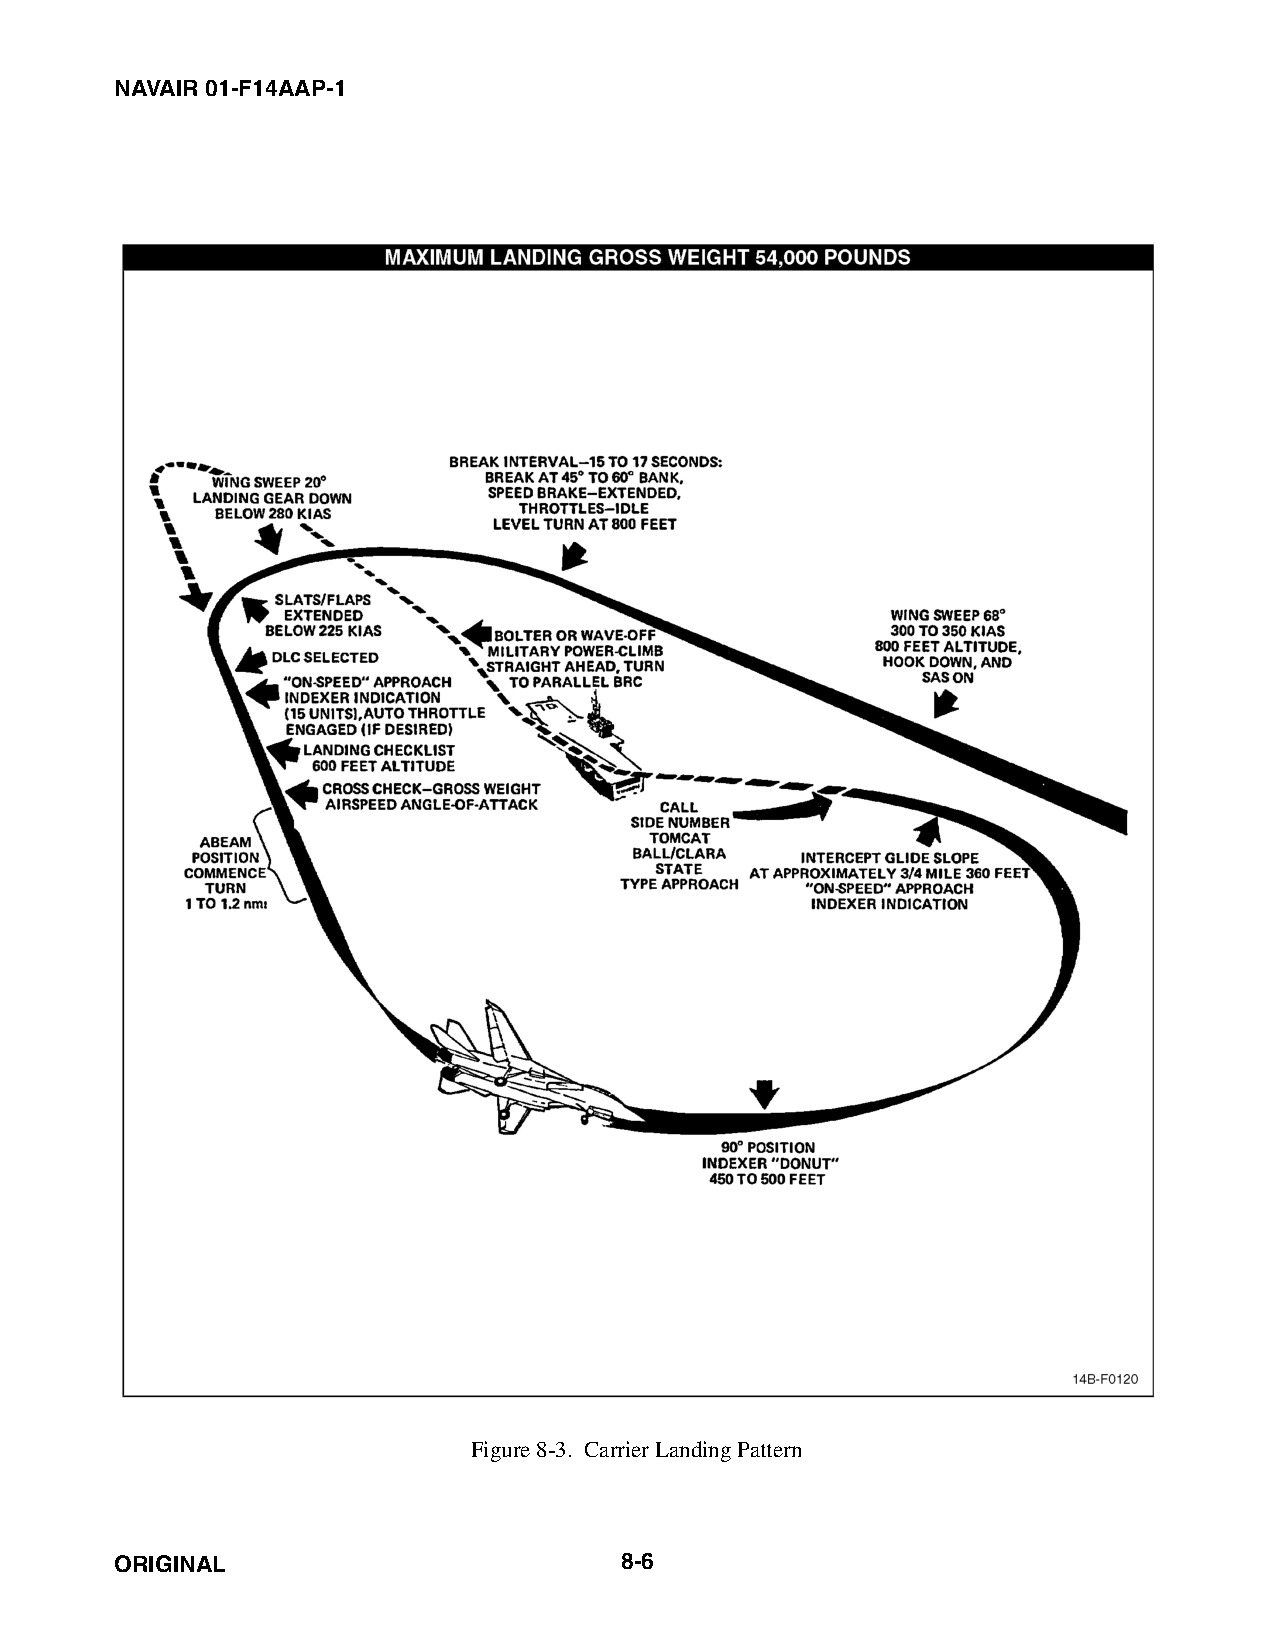
\includegraphics[
        width = 0.8\linewidth,
        page = {1},
        trim = {2.5cm, 7.5cm, 2.5cm, 7.5cm},
        clip
    ]{natops_F14B_case1.pdf}
    \caption{\textbf{Case I / Overhead Pattern}}
    \label{fig:case1}
\end{figure}

\begin{tablenumerate}
    \blueitem{Initial Approach}{
    \begin{subitemize}
        \item \textbf{WING SWEEP} \dotfill \textbf{68 deg}
        \item \textbf{HOOK} \dotfill \textbf{DOWN}
        \item \textbf{SAS} \dotfill \textbf{ON}
        \item \textbf{HUD} \dotfill \textbf{LDG}
        \item \textbf{Airspeed} \dotfill \textbf{300-350 KIAS}
        \item \textbf{Altitude} \dotfill \textbf{800 ft}
    \end{subitemize}}
    \blueitem{Initial Break}{
    \begin{subitemize}
        \item \textbf{Break Interval} \dotfill \textbf{15-17 s}
        \item \textbf{BANK} \dotfill \textbf{45-60 deg}
        \item \textbf{SPEED BRAKE} \dotfill \textbf{EXTEND}
        \item \textbf{Throttle} \dotfill \textbf{IDLE}
        \item \textbf{G} \dotfill \textbf{3-4 G}
        \item \textbf{Altitude} \dotfill \textbf{800 ft}
    \end{subitemize}}
    \blueitem{Break Turn}{
    \begin{subitemize}
        \item \textbf{Wing Sweep} \dotfill \textbf{AUTO} < 280 KIAS
        \item \textbf{Landing Gear} \dotfill \textbf{DOWN} < 280 KIAS
        \item \textbf{FLAPS} \dotfill \textbf{DOWN} < 225 KIAS
    \end{subitemize}}
    \blueitem{Downwind}{
    \begin{subitemize}
        \item \textbf{DLC} \dotfill \textbf{Selected} once flaps out
        \item \textbf{AOA} \dotfill \textbf{ON-SPEED}
        \item \hyperref[subsec:landchecklist]{\textbf{Landing Checklist}}
        \item \textbf{Altitude} \dotfill descend to \textbf{600 ft}
    \end{subitemize}}
    \blueitem{Final Turn}{\textbf{180 Deg Position}
    \begin{subitemize}
        \item \textbf{Abeam Pos.} \dotfill \textbf{1-1.2 nmi}
    \end{subitemize}
    \textbf{90 Deg Position}
    \begin{subitemize}
        \item \textbf{AOA} \dotfill \textbf{DONUT}
        \item \textbf{Altitude} \dotfill \textbf{400-500 ft}
    \end{subitemize}}
    \blueitem{Intercept \break Glideslope}{
    \begin{subitemize}
        \item \textbf{Distance} \dotfill \textbf{3/4 Mile}
        \item \textbf{Altitude} \dotfill \textbf{360 ft}
        \item \textbf{AOA} \dotfill \textbf{ON-SPEED}
    \end{subitemize}}
\end{tablenumerate}

\subsection{LANDING - CHECKLIST}
\label{subsec:landchecklist}
\begin{tablenumerate}
    \blueitem{Wing Sweep}{\textbf{20 deg AUTO}}
    \blueitem{Wheels}{
    \begin{subitemize}
        \item \textbf{Lights} \dotfill \textbf{3 DOWN}
        \item \textbf{Transition Light} \dotfill \textbf{OUT}
    \end{subitemize}}
    \blueitem{SAS}{\textbf{ON}}
    \blueitem{FLAPS}{\textbf{DOWN}}
    \blueitem{DLC}{\textbf{Checked}}
    \blueitem{Hook}{
    \begin{subitemize}
        \item \textbf{HOOK} \dotfill \textbf{DOWN}
        \item \textbf{Transition Light} \dotfill \textbf{OUT}
    \end{subitemize}}
    \blueitem{Harness}{\textbf{Locked}}
    \blueitem{Speedbrakes}{\textbf{EXT}}
    \blueitem{Brakes}{\textbf{Check}}
    \blueitem{Fuel}{\textbf{Check}}
\end{tablenumerate}

\clearpage

\subsection{LANDING - CASE III - ICLS}
\begin{tablenumerate}
    \blueitem{Inbound Call}{
    \begin{subenumerate}
        \item \textbf{UHF 1 \& V/UHF 2} \dotfill As Required 
        \item Contact Carrier and note QFE, Pattern Altitude, BRC
    \end{subenumerate}}
    \blueitem{Cockpit Check}{
    \begin{subenumerate}
        \item \textbf{Altimeter QFE} \dotfill \textbf{Set}
        \item \textbf{Cockpit Lighting} \dotfill As Desired 
        \item \textbf{Navigation Lights} \dotfill As Desired 
    \end{subenumerate}}
    \blueitem{Nav Systems}{
    \begin{subenumerate}
        \item \textbf{ARA-63} \dotfill \textbf{ON} \& tuned
        \item \textbf{TACAN} \dotfill \textbf{T/R} \& tuned
    \end{subenumerate}}
    \blueitem{Approach \break Navigation}{\emph{Use TACAN / ILS steering}

    \begin{subenumerate}
        \item \textbf{VDI Mode} \dotfill \textbf{NORM}
        \item \textbf{HSD Mode} \dotfill \textbf{NAV}
        \item \textbf{HUD Mode} \dotfill \textbf{LDG}
    \end{subenumerate}

    \emph{If ILS steering is desired must set AWL Mode}
    \begin{subenumerate}[start=4]
        \item \textbf{HUD AWL} \dotfill \textbf{ILS}
        \item \textbf{VDI AWL} \dotfill \textbf{ILS}
    \end{subenumerate}

    \emph{Set steering command to desired mode}
    \begin{subenumerate}[start=6]
        \item \textbf{STEER CMD} \dotfill \textbf{TACAN} or \textbf{AWL/PCD}
    \end{subenumerate}}
    \blueitem{Prepare Landing Systems}{
    \begin{subenumerate}
        \item \textbf{ANTI-SKID SPOILER BK} \dotfill \textbf{OFF}
        \item \textbf{HOOK BYPASS} \dotfill \textbf{CARRIER}
        \item \textbf{HOOK} \dotfill \textbf{DN}
        \item \textbf{WING SWEEP} \dotfill \textbf{AUTO}
        \item \textbf{SPEED BRAKE} \dotfill \textbf{OUT}
    \end{subenumerate}}
    \midrule
    \multicolumn{3}{l}{\textbf{25 NM FROM CARRIER}} \\
    \blueitem{Intercept Marshall Radial}{
    \begin{subitemize}
        \item \textbf{Range} -- 25nm 
        \item \textbf{Radial} -- Marshall Radial
        \item \textbf{Altitude} -- 10,000ft (descend to 5,000ft)
        \item \textbf{IAS} -- 250 kts
    \end{subitemize}}
    \midrule
    \multicolumn{3}{l}{\textbf{15 NM FROM CARRIER}} \\
    \blueitem{Intercept Runway Heading}{
    \begin{subitemize}
        \item \textbf{Range} -- Maintain 15nm during turn
        \item \textbf{Radial} -- Runway Heading
        \item \textbf{Altitude} -- Maintain 5,000ft
        \item \textbf{IAS} -- 250 kts
    \end{subitemize}}
    \blueitem{ILS Steering}{
    \begin{subenumerate}
        \item \textbf{STEER CMD} \dotfill \textbf{AWL/PCD}
        \item \textbf{HUD AWL} \dotfill \textbf{ILS}
        \item \textbf{VDI AWL} \dotfill \textbf{ILS}
    \end{subenumerate}}
    \midrule
    \multicolumn{3}{l}{\textbf{10 NM FROM CARRIER}} \\
    \blueitem{Landing \break Configuration}{
    \begin{subenumerate}
        \item \textbf{HOOK} \dotfill \textbf{DN}
        \item \textbf{SPEED BRAKE} \dotfill \textbf{OUT}
        \item \textbf{WING SWEEP} \dotfill \textbf{20deg AUTO}
        \item \textbf{GEAR} \dotfill \textbf{Down}
        \item \textbf{FLAPS} \dotfill \textbf{Full}
        \item \textbf{Autothrottle} \dotfill \textbf{AUTO} \\
        \hfill (if desired)
        \item \textbf{AOA} \dotfill \textbf{ON-SPEED} \\
        \hfill (Autothrottle should maintain On-Speed)
    \end{subenumerate}}
    \blueitem{FINAL}{
    \begin{subenumerate}
        \item \textbf{Follow ICLS Needles}
        \item \textbf{Transition to flying the ball once visual}
    \end{subenumerate}}
\end{tablenumerate}

\notebox{
    \begin{itemize}
        \item \textbf{APC does NOT advance throttle on touchdown}
        \item \hyperref[tab:vdicautionind]{\textbf{Refer to VDI Caution Indicator Table for summary}}
    \end{itemize}
}

\clearpage

\subsection{LANDING - CASE III - ACLS}
\begin{tablenumerate}
    \blueitem{Inbound Call}{
    \begin{subenumerate}
        \item \textbf{UHF 1 \& V/UHF 2} \dotfill As Required 
        \item Contact Carrier and note QFE, Pattern Altitude, BRC
    \end{subenumerate}}
    \blueitem{Cockpit Check}{
    \begin{subenumerate}
        \item \textbf{Altimeter QFE} \dotfill \textbf{Set}
        \item \textbf{Cockpit Lighting} \dotfill As Desired 
        \item \textbf{Navigation Lights} \dotfill As Desired 
    \end{subenumerate}}
    \blueitem{Nav Systems}{
    \begin{subenumerate}
        \item \textbf{ARA-63} \dotfill \textbf{ON} \& tuned
        \item \textbf{TACAN} \dotfill \textbf{T/R} \& tuned
    \end{subenumerate}}
    \blueitem{Approach \break Navigation}{\emph{Use TACAN / ILS steering to follow approach pattern before engaging ACLS on final}

    \begin{subenumerate}
        \item \textbf{VDI Mode} \dotfill \textbf{NORM}
        \item \textbf{HSD Mode} \dotfill \textbf{NAV}
        \item \textbf{HUD Mode} \dotfill \textbf{LDG}
    \end{subenumerate}

    \emph{If ILS steering is desired must set AWL Mode}
    \begin{subenumerate}[start=4]
        \item \textbf{HUD AWL} \dotfill \textbf{ILS}
        \item \textbf{VDI AWL} \dotfill \textbf{ILS}
    \end{subenumerate}

    \emph{Set steering command to desired mode}
    \begin{subenumerate}[start=6]
        \item \textbf{STEER CMD} \dotfill \textbf{TACAN} or \textbf{AWL/PCD}
    \end{subenumerate}}
    \dblueitem{ACLS Setup}{
    \begin{subenumerate}
        \item \textbf{DL Power} \dotfill \textbf{ON}
        \item \textbf{DL Mode} \dotfill \textbf{TAC}
        \item \textbf{DL Freq.} \dotfill As Required
        \item \textbf{APN-154 Power} \dotfill \textbf{ON}
        \item \textbf{ACLS TEST Light} \dotfill Verify ON
    \end{subenumerate}}
    \blueitem{Prepare Landing Systems}{
    \begin{subenumerate}
        \item \textbf{ANTI-SKID SPOILER BK} \dotfill \textbf{OFF}
        \item \textbf{HOOK BYPASS} \dotfill \textbf{CARRIER}
        \item \textbf{HOOK} \dotfill \textbf{DN}
        \item \textbf{WING SWEEP} \dotfill \textbf{AUTO}
        \item \textbf{SPEED BRAKE} \dotfill \textbf{OUT}
    \end{subenumerate}}
    \midrule
    \multicolumn{3}{l}{\textbf{25 NM FROM CARRIER}} \\
    \blueitem{Intercept Marshall Radial}{
    \begin{subitemize}
        \item \textbf{Range} -- 25nm 
        \item \textbf{Radial} -- Marshall Radial
        \item \textbf{Altitude} -- 10,000ft (descend to 5,000ft)
        \item \textbf{IAS} -- 250 kts
    \end{subitemize}}
    \midrule
    \multicolumn{3}{l}{\textbf{15 NM FROM CARRIER}} \\
    \blueitem{Intercept Runway Heading}{
    \begin{subitemize}
        \item \textbf{Range} -- Maintain 15nm during turn
        \item \textbf{Radial} -- Runway Heading
        \item \textbf{Altitude} -- Maintain 5,000ft
        \item \textbf{IAS} -- 250 kts
    \end{subitemize}}
    \blueitem{Autopilot Setup}{
    \begin{subenumerate}
        \item \textbf{STEER CMD} \dotfill \textbf{AWL/PCD}
        \item \textbf{HUD AWL} \dotfill \textbf{ACL}
        \item \textbf{VDI AWL} \dotfill \textbf{ACL}
        \item \textbf{Autopilot Selector} \dotfill \textbf{ACL}
        \item \textbf{Autopilot Switch} \dotfill \textbf{ENGAGE}
        \item \textbf{A/P REF Light} \dotfill Verify Illuminates \\
        \hfill (autopilot ready for activation)
        \item \textbf{Autothrottle} \dotfill \textbf{AUTO}
    \end{subenumerate}}
    \midrule
    \multicolumn{3}{l}{\textbf{10 NM FROM CARRIER}} \\
    \blueitem{Landing \break Configuration}{
    \begin{subenumerate}
        \item \textbf{HOOK} \dotfill \textbf{DN}
        \item \textbf{SPEED BRAKE} \dotfill \textbf{OUT}
        \item \textbf{WING SWEEP} \dotfill \textbf{20deg AUTO}
        \item \textbf{GEAR} \dotfill \textbf{Down}
        \item \textbf{FLAPS} \dotfill \textbf{Full}
        \item \textbf{AOA} \dotfill \textbf{ON-SPEED} \\
        \hfill (Autothrottle should maintain On-Speed)
    \end{subenumerate}}
    \blueitem{FINAL}{
    \begin{subenumerate}
        \item \textbf{LANDING CHK Caution} \dotfill Illuminates (6nm)
        \item \textbf{ACL READY Caution} \dotfill Illuminates (4nm)
        \item \textbf{AP/CPLR Caution} \dotfill Illuminates \\
        \hfill (Indicates Carrier ready to control A/C)
        \begin{itemize}
            \item \textbf{Localizer Needle} -- Verify Centered
            \item \textbf{Glideslope Needle} -- Verify Centered
        \end{itemize}
        \item \textbf{Autopilot Reference} \dotfill \textbf{Depress}
        \item \textbf{CMD CONTROL Caution} \dotfill Illuminates
        \item \textbf{10 SECONDS Caution} \dotfill Illuminates \\
        \hfill Prior to touchdown
    \end{subenumerate}}
\end{tablenumerate}

\notebox{
    \begin{itemize}
        \item \textbf{Pilot should be ready to disengage ACLS at any time}
        \begin{itemize}
            \item Can be disengaged with \textbf{PLM Depress}
        \end{itemize}
        \item \textbf{APC does NOT advance throttle on touchdown}
        \item \hyperref[tab:vdicautionind]{\textbf{Refer to VDI Caution Indicator Table for summary}}
    \end{itemize}
}

\begin{table}[h]
    \caption{\textbf{VDI Caution Indicators}}
    \label{tab:vdicautionind}
    \begin{tabular}{p{2.8cm} | p{9cm}}
        \toprule
        \blue{Light} & \blue{Description} \\
        \midrule
        \textbf{ADJ A/C} & Indicates other aircraft close to own traffic pattern \\
        \midrule
        \textbf{LANDING CHK} & Indicates carrier has channel ready for ACL, crew should prepare for carrier landing, center needles \\
        \midrule
        \textbf{ACL READY} & Indicates CATCC has aquired aircraft and is transmitting glidepath information \\
        \midrule
        \textbf{A/P CPLR} & Indicates CATCC is ready to control aircraft \\
        \midrule
        \textbf{CMD CONTROL} & Indicates aircraft is under data link control for landing \\
        \midrule
        \textbf{10 SECONDS} & Indicates that carrier motion is added to data link info and commands during landing \\
        & Indicates 10 seconds to arrival at the next point in approach pattern in other modes \\
        \midrule
        \textbf{TILT} & Caution that data link command received for the last 2 seconds during ACL \\
        & When not in ACL it indicates no data link messages during last 10 seconds \\
        \midrule
        \textbf{VOICE} & Caution that CATCC not ready for ACL, switch to standard voice procedures \\
        \midrule
        \textbf{AUTO THRO} & Caution that autothrottle has been disengaged \\
        \midrule
        \textbf{A/P REF} & Indicates autopilot selected but not engaged. Exception altitude and heading hold \\
        \midrule
        \textbf{WAVEOFF} & Indicates waveoff commanded \\
        \midrule
        \textbf{WING SWEEP} & Caution indicating failure in both wing-sweep channels or disengagement of spider detent \\
        \midrule
        \textbf{REDUCE SPEED} & Indicates flap retraction failure with greater than 225 knots indicated airspeed \\
        & Also indicates safe Mach number exceeded \\
        \midrule
        \textbf{ALT LOW} & Non functional, refer to radar altimeter \\
        \bottomrule
    \end{tabular}
\end{table}

\clearpage

\section{IN-FLIGHT}
\subsection{AERIAL REFUELING}
\begin{tablenumerate}
    \blueitem{REFUELING CHECKLIST}{
    \begin{subenumerate}
        \item \textbf{WCS} \dotfill \textbf{STBY}
        \item \textbf{ARMING} \dotfill \textbf{SAFE}
        \item \textbf{DUMP Switch} \dotfill \textbf{OFF}
        \item \textbf{AIR SOURCE} \dotfill \textbf{L ENG}
        \item \textbf{REFUEL PROBE} \dotfill \textbf{As desired} \\
        \hfill (transition light off)
        \item \textbf{WING SWEEP} \dotfill \textbf{As desired}
    \end{subenumerate}}
    \blueitem{DISENGAGEMENT}{
    \begin{subenumerate}
        \item \textbf{REFUEL PROBE} \dotfill \textbf{RET} \\
        \hfill (transition light off)
        \item \textbf{AIR SOURCE} \dotfill \textbf{BOTH}
        \item \textbf{WING SWEEP} \dotfill \textbf{AUTO}
    \end{subenumerate}}
\end{tablenumerate}

\clearpage

\section{EMERGENCY PROCEDURES}

\subsection{AIRSTART}
\begin{tableitemize}
    \blueitem{Spooldown}{\emph{Before significant spooldown}
    \begin{subenumerate}
        \item \textbf{Non-Running ENG} \dotfill \textbf{IDLE} or above
    \end{subenumerate}

    \emph{If no relight occurs}
    \begin{subenumerate}[start=2]
        \item \textbf{Non-Running ENG} \dotfill \textbf{OFF} then \textbf{IDLE}
    \end{subenumerate}

    \emph{If still no relight occurs}
    \begin{subenumerate}[start=3]
        \item \textbf{ENG MODE} \dotfill \textbf{SEC}
        \item \textbf{Non-Running ENG} \dotfill \textbf{OFF} then \textbf{IDLE}
    \end{subenumerate}}
    \blueitem{Cross-Bleed Restart}{
    \emph{With one ENG running, if Spooldown fails}
    \begin{subenumerate}
        \item \textbf{Non-Running ENG} \dotfill \textbf{OFF}
        \item \textbf{FUEL SHUT OFF} \dotfill check
        \item \textbf{Running throttle} \dotfill 80\%+
        \item \textbf{BACK UP IGNITION} \dotfill \textbf{ON}
        \item \textbf{ENG CRANK} \dotfill non-running eng
        \item \textbf{Non-Running ENG} \dotfill \textbf{IDLE}
    \end{subenumerate}

    \emph{If no start occurs}
    \begin{subenumerate}[start=7]
        \item \textbf{Non-Running ENG} \dotfill \textbf{OFF} then \textbf{IDLE}
    \end{subenumerate}

    \emph{If still no start}
    \begin{subenumerate}[start=8]
        \item \textbf{ENG MODE} \dotfill \textbf{SEC}
        \item \textbf{Non-Running ENG} \dotfill \textbf{OFF} then \textbf{IDLE}
    \end{subenumerate}}
    \blueitem{Windmill Restart}{
    \begin{subenumerate}
        \item \textbf{Airspeed} \dotfill >450 kts
        \item \textbf{Throttle} \dotfill IDLE or above
        \item \textbf{BACK UP IGNITION} \dotfill ON
    \end{subenumerate}

    \emph{If no relight occurs}
    \begin{subenumerate}[start=4]
        \item \textbf{Throttle} \dotfill OFF then IDLE
    \end{subenumerate}

    \emph{If still no relight}
    \begin{subenumerate}[start=5]
        \item \textbf{ENG MODE} \dotfill SEC
        \item \textbf{Throttle} \dotfill OFF then IDLE
    \end{subenumerate}}
    \blueitem{Post Restart}{
    \begin{subenumerate}
            \item \textbf{BACK UP IGNITION} \dotfill OFF
            \item \textbf{ENG MODE} \dotfill PRI
        \end{subenumerate}}
\end{tableitemize}

\cleardoublepage